\documentclass[xcolor=dvipsnames, USenglish]{beamer}  %notes=show to print them in the generated pdf
% Packages for a reasonable beamer session
\usepackage[T1]{fontenc}
%\usepackage[ansinew]{inputenc}
\usepackage[utf8]{inputenc}
\usepackage{textcomp}
\usepackage{lmodern}
\usepackage{csquotes}
\usepackage[english]{babel}
%\usepackage{babel}

\usepackage{graphicx}

\usepackage{amsmath}
\usepackage{amsfonts}
\usepackage{amssymb}
\usepackage{amsthm}
\usepackage{bm}

\usepackage{booktabs}
\usepackage{tabularx}

\usepackage{hyperref}

\usepackage{ellipsis}

% Additional packages
\usepackage{graphicx}
\usepackage{subfigure}
\usepackage{xcolor}
\usepackage{minted}

\usepackage[style=authoryear, backend=biber]{biblatex}
\setbeamertemplate{itemize/enumerate body begin}{\setlength{\leftmargini}{1.5em}}
\renewcommand*{\nameyeardelim}{\addcomma\addspace}
\addbibresource{\jobname.bib}
\renewcommand{\footnotesize}{\tiny}

\usepackage{tikz,pgf,calc}
%\usetikzlibrary{matrix, shapes, positioning, calc,
%  decorations.pathreplacing, shapes.geometric, arrows}
\usetikzlibrary{shapes.geometric, arrows, calc}
\tikzstyle{startstop} = [rectangle, rounded corners, minimum width=3cm, minimum height=1cm, text centered, text width=1.5cm, draw=black, fill=red!30]
\tikzstyle{io} = [trapezium, trapezium left angle=70, trapezium right angle=110, minimum width=3cm, minimum height=1cm, text centered, draw=black, fill=blue!30]
\tikzstyle{process} = [rectangle, minimum width=3cm, minimum height=1cm, text centered, draw=black, fill=orange!30]
\tikzstyle{decision} = [diamond, minimum width=3cm, minimum height=0.5cm, text centered, draw=black, fill=green!30]
\tikzstyle{arrow} = [thick,->,>=stealth]

%% References
\newlength\leftsidebar
\makeatletter
\setlength\leftsidebar{\beamer@leftsidebar}
\makeatother

\usepackage[absolute,overlay]{textpos}
\newenvironment{reference}[2]{%
  \begin{textblock*}{\textwidth}(\leftsidebar+#1,\paperheight-#2)
      \scriptsize\bgroup\color{red!50!black}}{\egroup\end{textblock*}}

% Path to graphics
\graphicspath{{../img/}}

% Sources
\usepackage{setspace}
\newcommand{\source}[1]{\begin{spacing}{0.5}{\fontsize{5}{6}\selectfont source: \itshape {#1}}\end{spacing}}
 % PACKAGES
% Collection of useful mathematical symbols and commands
% Calculus
\newcommand{\ud}{\mathrm{d}}
\newcommand{\pder}[2]{\frac{\partial{#1}}{\partial{#2}}}
\newcommand{\dpder}[2]{\frac{\partial^2{#1}}{\partial{#2^2}}}
\newcommand{\sderp}[3]{\frac{\partial^2{#1}}{\partial{#2}\partial{#3}}}
\newcommand{\tder}[2]{\frac{\ud{#1}}{\ud{#2}}}
\newcommand{\rot}[1]{\nabla \times {#1}}
\newcommand{\diver}[1]{\nabla \cdot {#1}}
\newcommand{\definter}[4]{\int_{#1}^{#2} {#3}\ud {#4}}
\newcommand{\inter}[2]{\int {#1}\ud {#2}}
\newcommand{\braket}[2]{\langle {#1} , {#2} \rangle}
% Misc
\newcommand{\eval}[1]{\Big |_{#1}}
\newcommand{\bset}[1]{\big\lbrace {#1} \big\rbrace}
\newcommand{\stimes}[2]{{#1}\!\times\!{#2}}
\newcommand{\trp}{\top}
\newcommand{\preup}[2]{{}^{#2}\!{#1}}

% Operators
\DeclareMathOperator*{\armin}{arg\,min}
\DeclareMathOperator*{\armax}{arg\,max}
\DeclareMathOperator*{\rank}{rank}
\DeclareMathOperator*{\cov}{cov}
\DeclareMathOperator*{\nullsp}{null}
% Logicals
\newcommand{\suchthat}{\big \backslash \;}
   % SYMBOLS

% ----------- extra packages
\usepackage{../beamer_themes/beamerthemeEawag_blue} % Eawag style

% ----------- Extra symbols
\newcommand{\ccov}[1]{{\color{red}k}\left(#1\right)}
\newcommand{\cmean}[1]{{\color{blue}m}\left(#1\right)}
\newcommand{\sm}{\scalebox{0.5}{-1}}

% ----------- For boxed equations
\usepackage{amsmath}
\usepackage{empheq}
\usepackage[most]{tcolorbox}
\newtcbox{\mymath}[1][]{%
    nobeforeafter, math upper, tcbox raise base,
    enhanced, colframe=blue!30!black,
    colback=blue!30, boxrule=1pt,
    #1}



%----------------
% title information
\title{Master Thesis - Presentation 2}
\subtitle{Development of an Overland Flow Model Emulator}
\author[\texttt{sebastiano.rusca@eawag.ch}]{Sebastiano Rusca}
\institute[Eawag]{Eawag: Swiss Federal Institute of Aquatic Science
  and Technology}
\date[07.02.2018]{Februar 07, 2018}

% ====================================================================

\begin{document}

% ----------------
% Title frame
% load background for title
\setbeamertemplate{background}{
  
\includegraphics[width=\paperwidth,height=\paperheight]
  {../beamer_themes/background_title_blue.png}}
{ \setbeamertemplate{footline}{} % no footer on title
  \begin{frame}
    \titlepage
  \end{frame}
}
% load background for all other slides
\setbeamertemplate{background}{

\includegraphics[width=\paperwidth,height=\paperheight]
{../beamer_themes/background_slides_blue.png}}
\setbeamertemplate{footline}[Sebastiano Rusca] % set footer
\addtocounter{framenumber}{-1}  % don't count title page

%%%%%%%%%%%%%%%%%%%%%%%%%%%%%%%%%%%%%%%%%%%%%%%
%----------------
\section{Introduction}

  \begin{frame}
    \frametitle{Outline}
    \begin{itemize}
      \item \textbf{Task 1}: channel flow simulations
        \begin{itemize} 
          \item derivation of the weir equation from numerical simulations
        \end{itemize}
      \item \textbf{Preparation}: learning of different interpolation techniques
      \item \textbf{Task 2}: hydrological simulations
        \begin{itemize}
          \item run simulations
          \item extract outputs
          \item build emulator (inputs -- outputs)
        \end{itemize}
     \end{itemize}
     \note{write your notes here. Set "notes=show" to print them in the pdf}
  \end{frame}

%%%%%%%%%%%%%%%%%%%%%%%%%%%%%%%%%%%%%%%%%%%%%%%%%%%%%%%%%%%%%%%%%%%%%%%%%%%%%%%%
% TASK 1 - Weir equation from numerical experiments: Setup

\section{Task 1}

  \begin{frame}
    \frametitle{Task 1 - Learning the weir equation}
    \centering
    \begin{empheq}[box=\tcbhighmath]{equation*}
      Q = \frac{2}{3}\: \textcolor{blue}{\mu}\: B_w\: \sqrt{2g}\: h_{\"u}^{\textcolor{blue}{a}}, \quad usu.\: \textcolor{blue}{a = 3/2}
    \end{empheq}

    \begin{figure}[H]
      \centering
      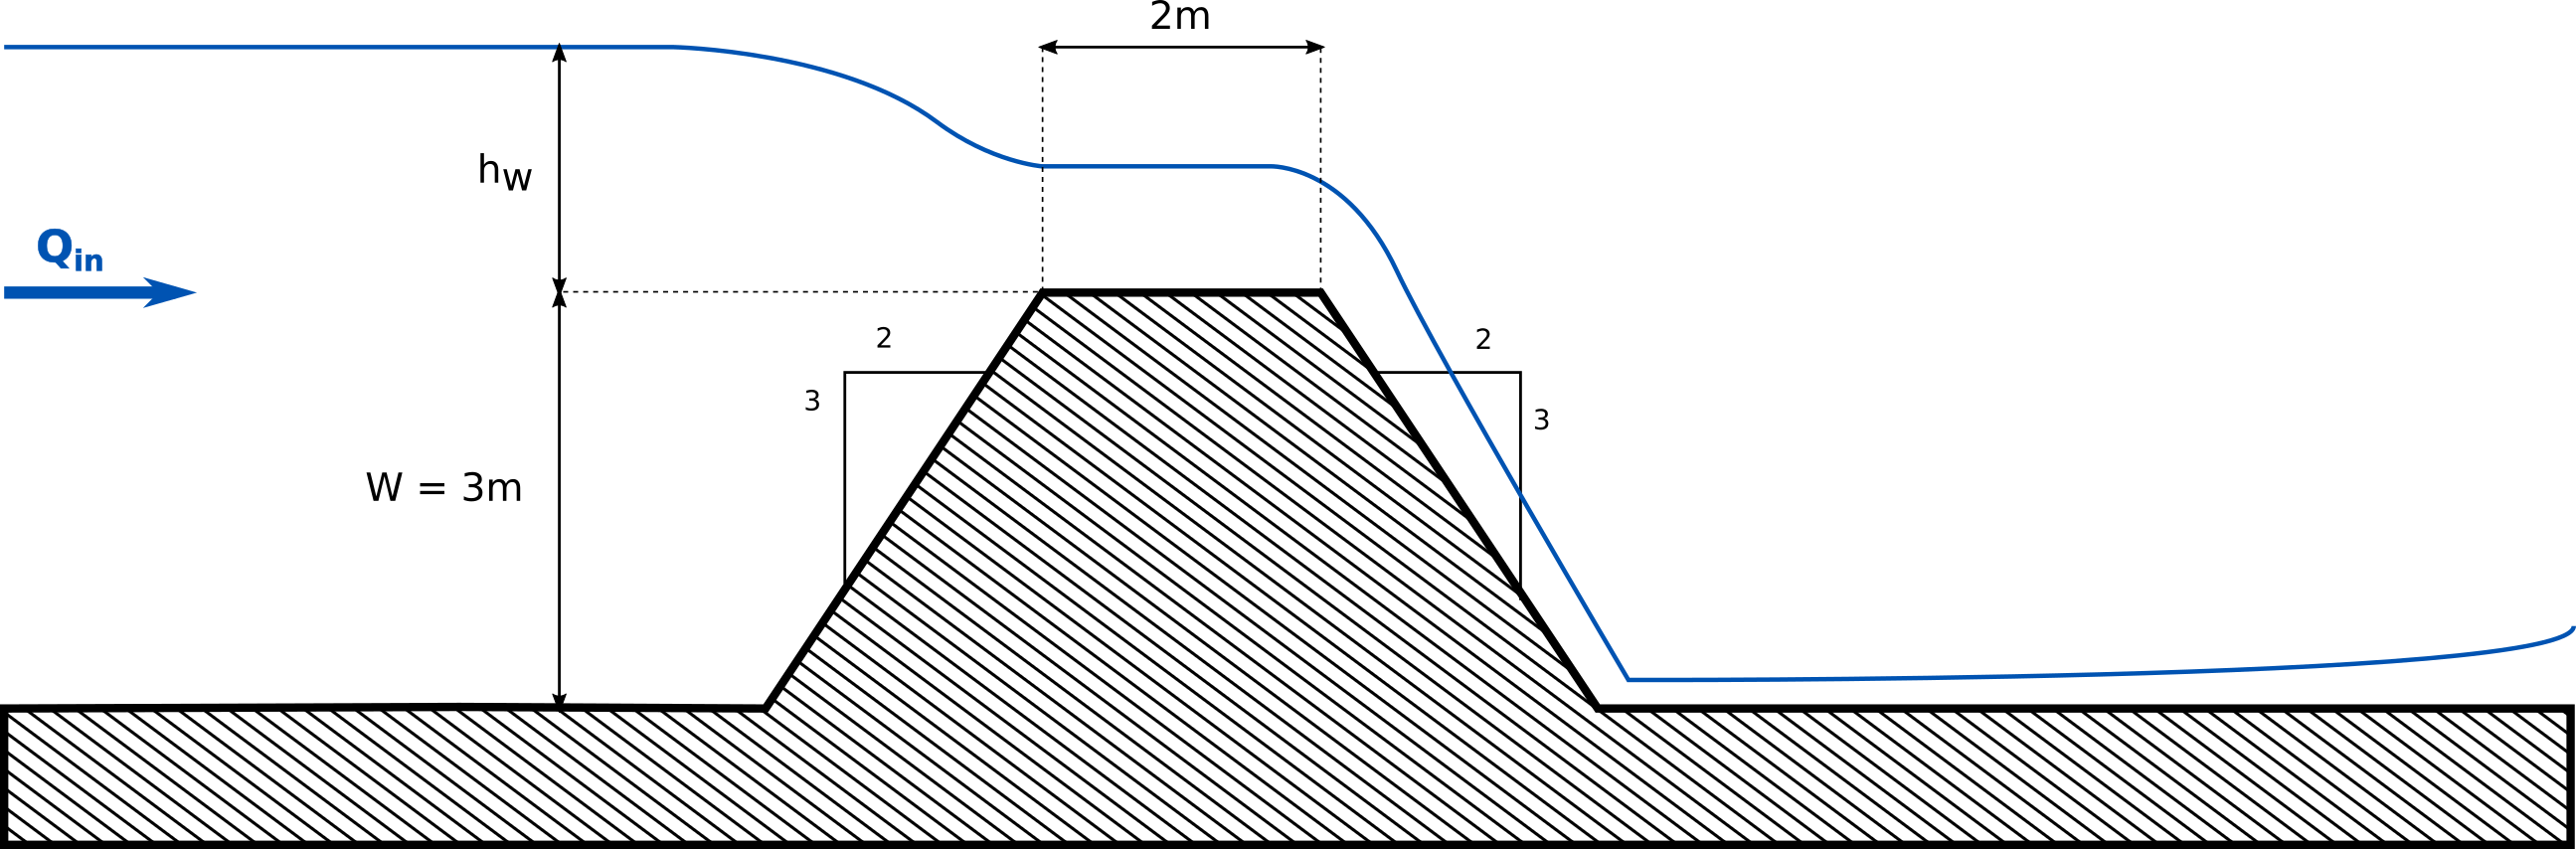
\includegraphics[width=0.7\textwidth]{img/weir.png}
      \\
      $\boldsymbol{\mu:}$ \raisebox{-.2\height}{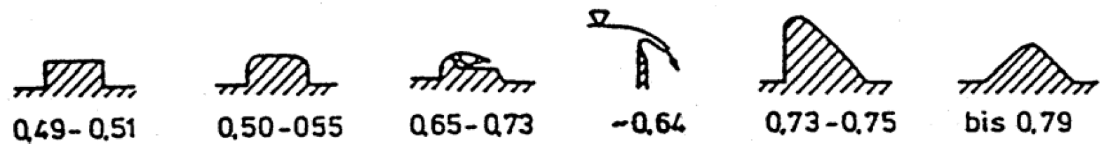
\includegraphics[width=0.6\textwidth]{img/weir_coefficients.png}}
    \end{figure}
    \source{Boes, Robert. "Wasserbau - Vorlesungsmanuskript." ETH Z\"urich - VAW, 2016.}
  \end{frame}

%%%%%%%%%%%%%%%%%%%%%%%%%%%%%%%%%%%%%%%%%%%%%%%%%%%%%%%%%%%%%%%%%%%%%%%%%%%%%%%%
% TASK 1 - Weir equation from numerical experiments: Results

\section{Task 1}
  \begin{frame}
    \frametitle{Task 1 - Results}
    \centering
    \begin{figure}[t]
      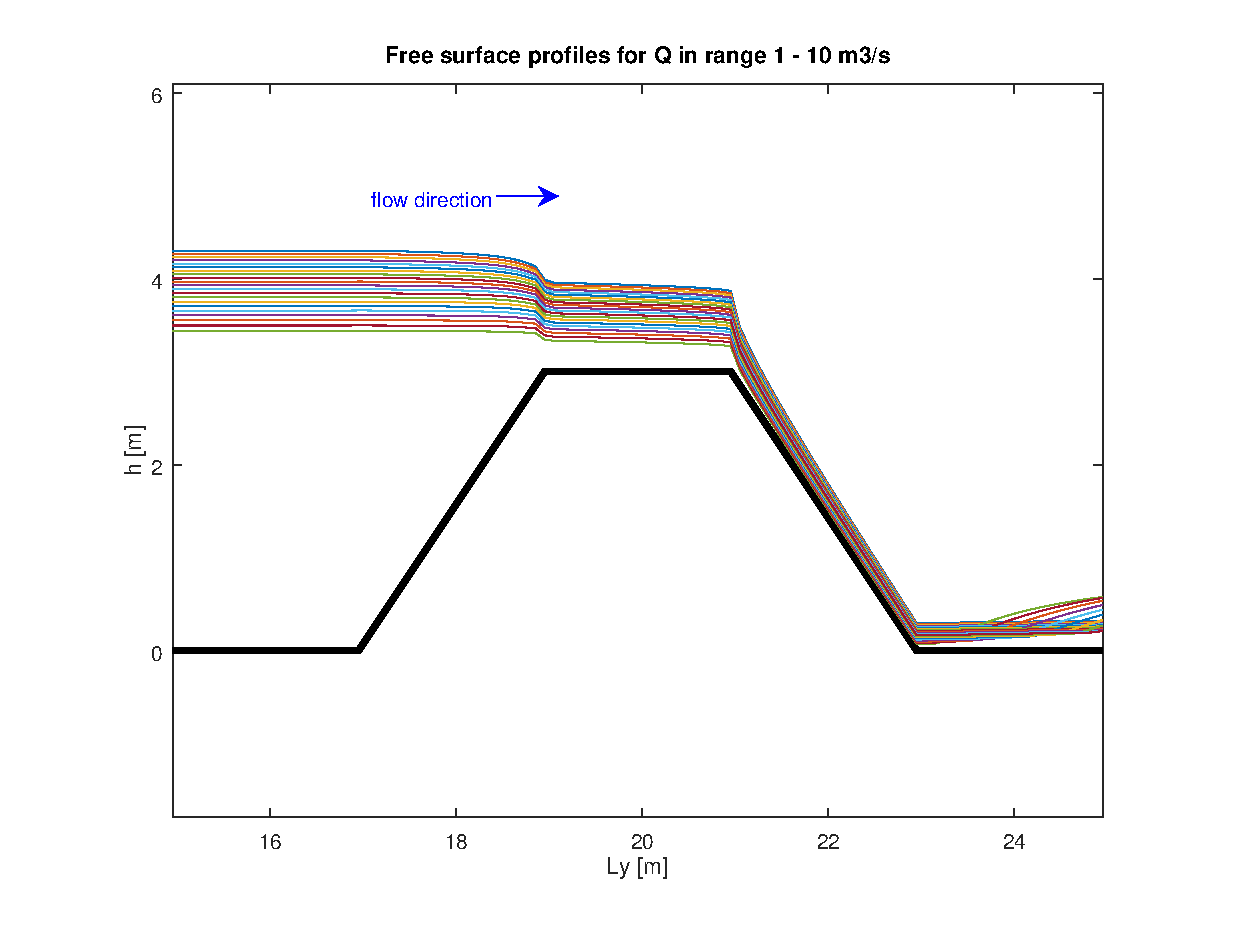
\includegraphics[width=0.5\textwidth]{img/free_surfaces.eps}
      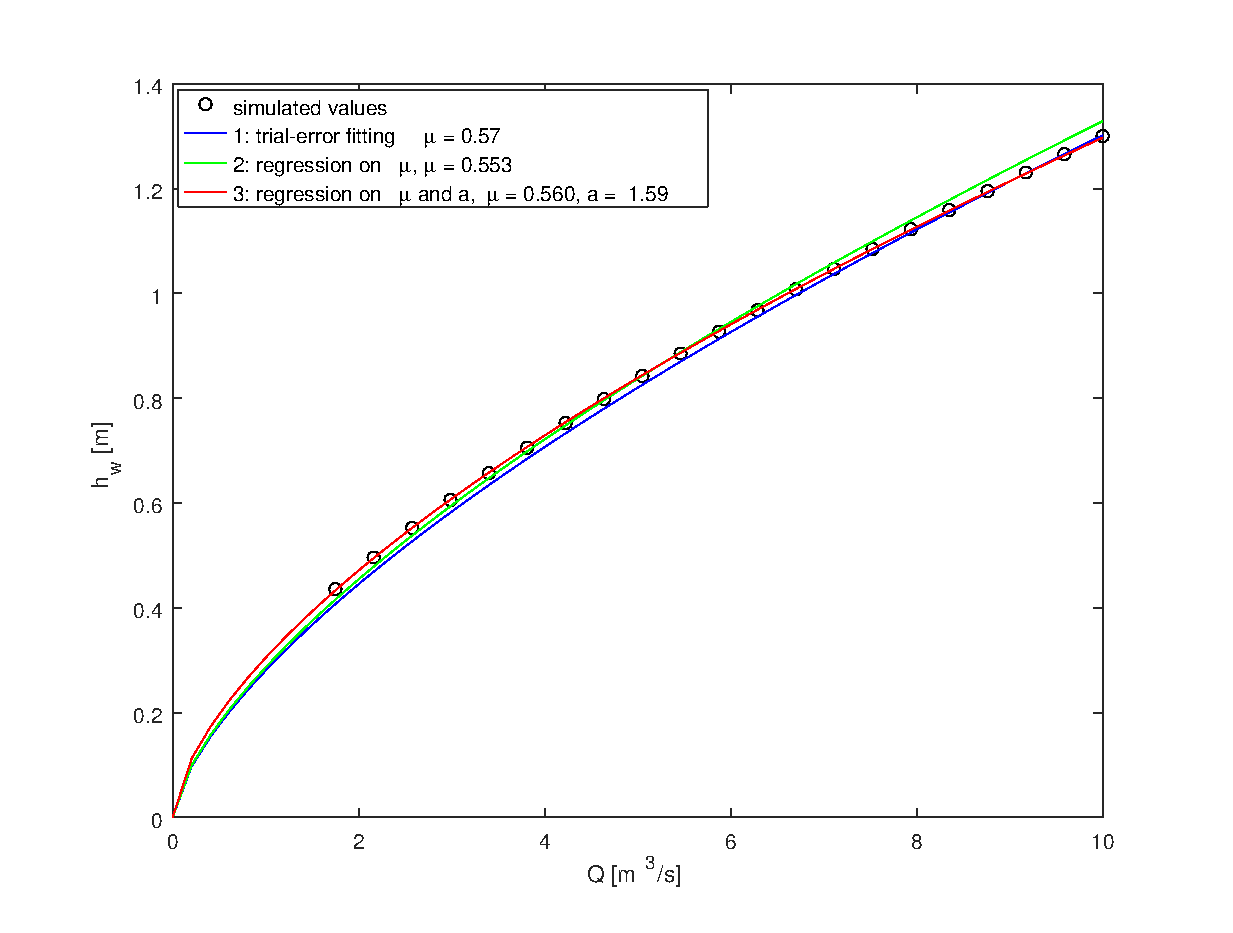
\includegraphics[width=0.5\textwidth]{img/points_interpolations.eps}
    \end{figure}

    \begin{table}
    \centering
       \begin{tabular}{lccc}
       \toprule
       \textbf{fitting method} & $\boldsymbol{\mu}$ &  \textbf{a} & \textbf{MSE}\\
       \midrule
       1: trial-error & 0.570 & 1.50 & 2.69E-04\\
       2: regression on $\mu$ & 0.553 & 1.50 & 2.36E-04\\
       3: regression on $\mu$ and a & 0.560 & 1.59 & 2.25E-06\\
       \bottomrule
       \end{tabular}
    \end{table}
  \end{frame}

%%%%%%%%%%%%%%%%%%%%%%%%%%%%%%%%%%%%%%%%%%%%%%%%%%%%%%%%%%%%%%%%%%%%%%%%%%%%%%%%
% PREPARATION TASK 2 - Interpolation exercises

\section{Task 2 - Preparation}
  \begin{frame}
    \frametitle{Preparation - Interpolation methods}
    \large{\textbf{Polynomial interpolation}}\\
    \begin{figure}[t]
      \centering
      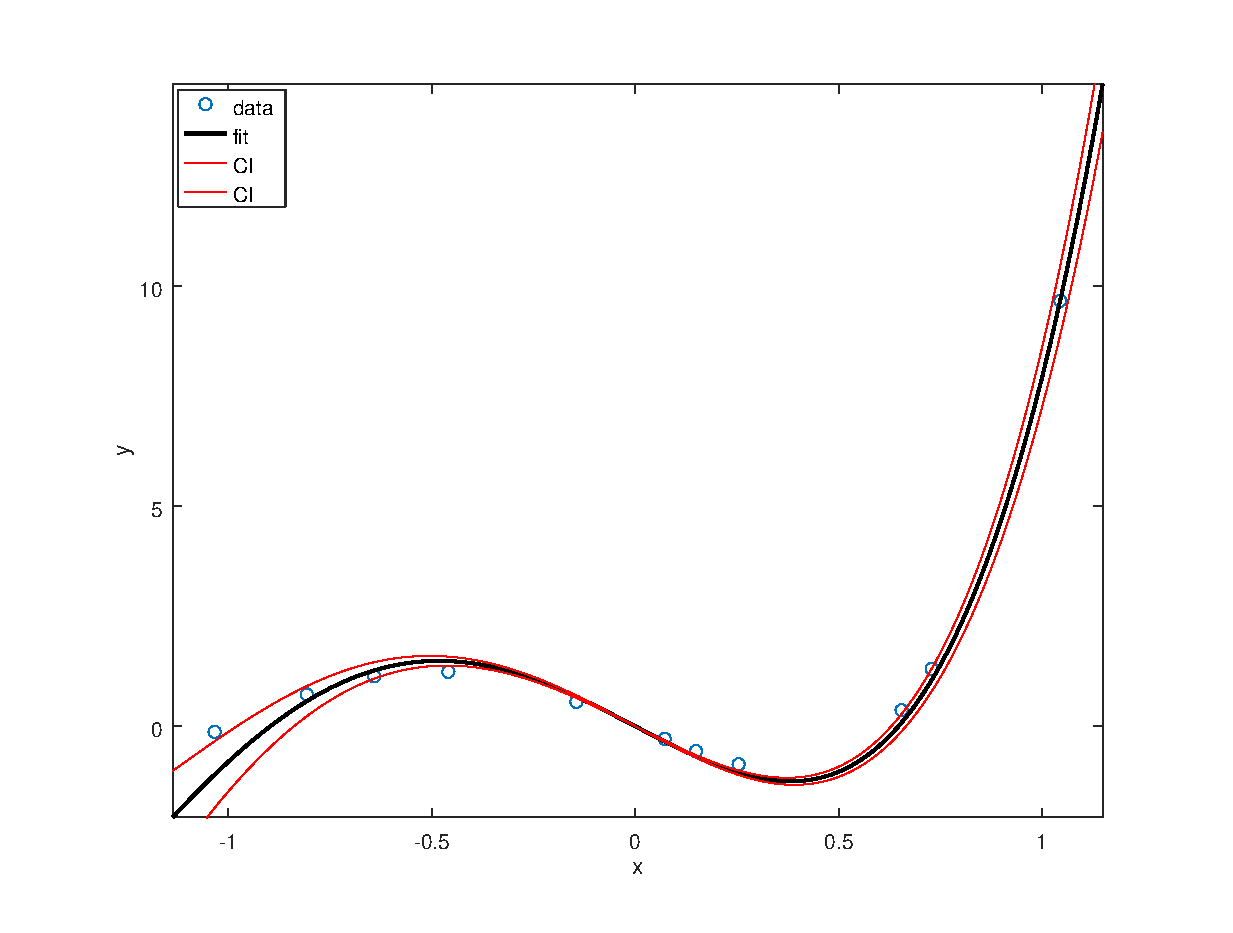
\includegraphics[width=0.7\textwidth]{img/interpolation.eps}
    \end{figure}
  \end{frame}

%%%%%%%%%%%%%%%%%%%%%%%%%%%%%%%%%%%%%%%%%%%%%%%%%%%%%%%%%%%%%%%%%%%%%%%%%%%%%%%%
% TASK 2 - Set-up

\section{Task 2}
  \begin{frame}
    \frametitle{Task 2 - Set-up}
    \begin{figure}[t]
      \centering
      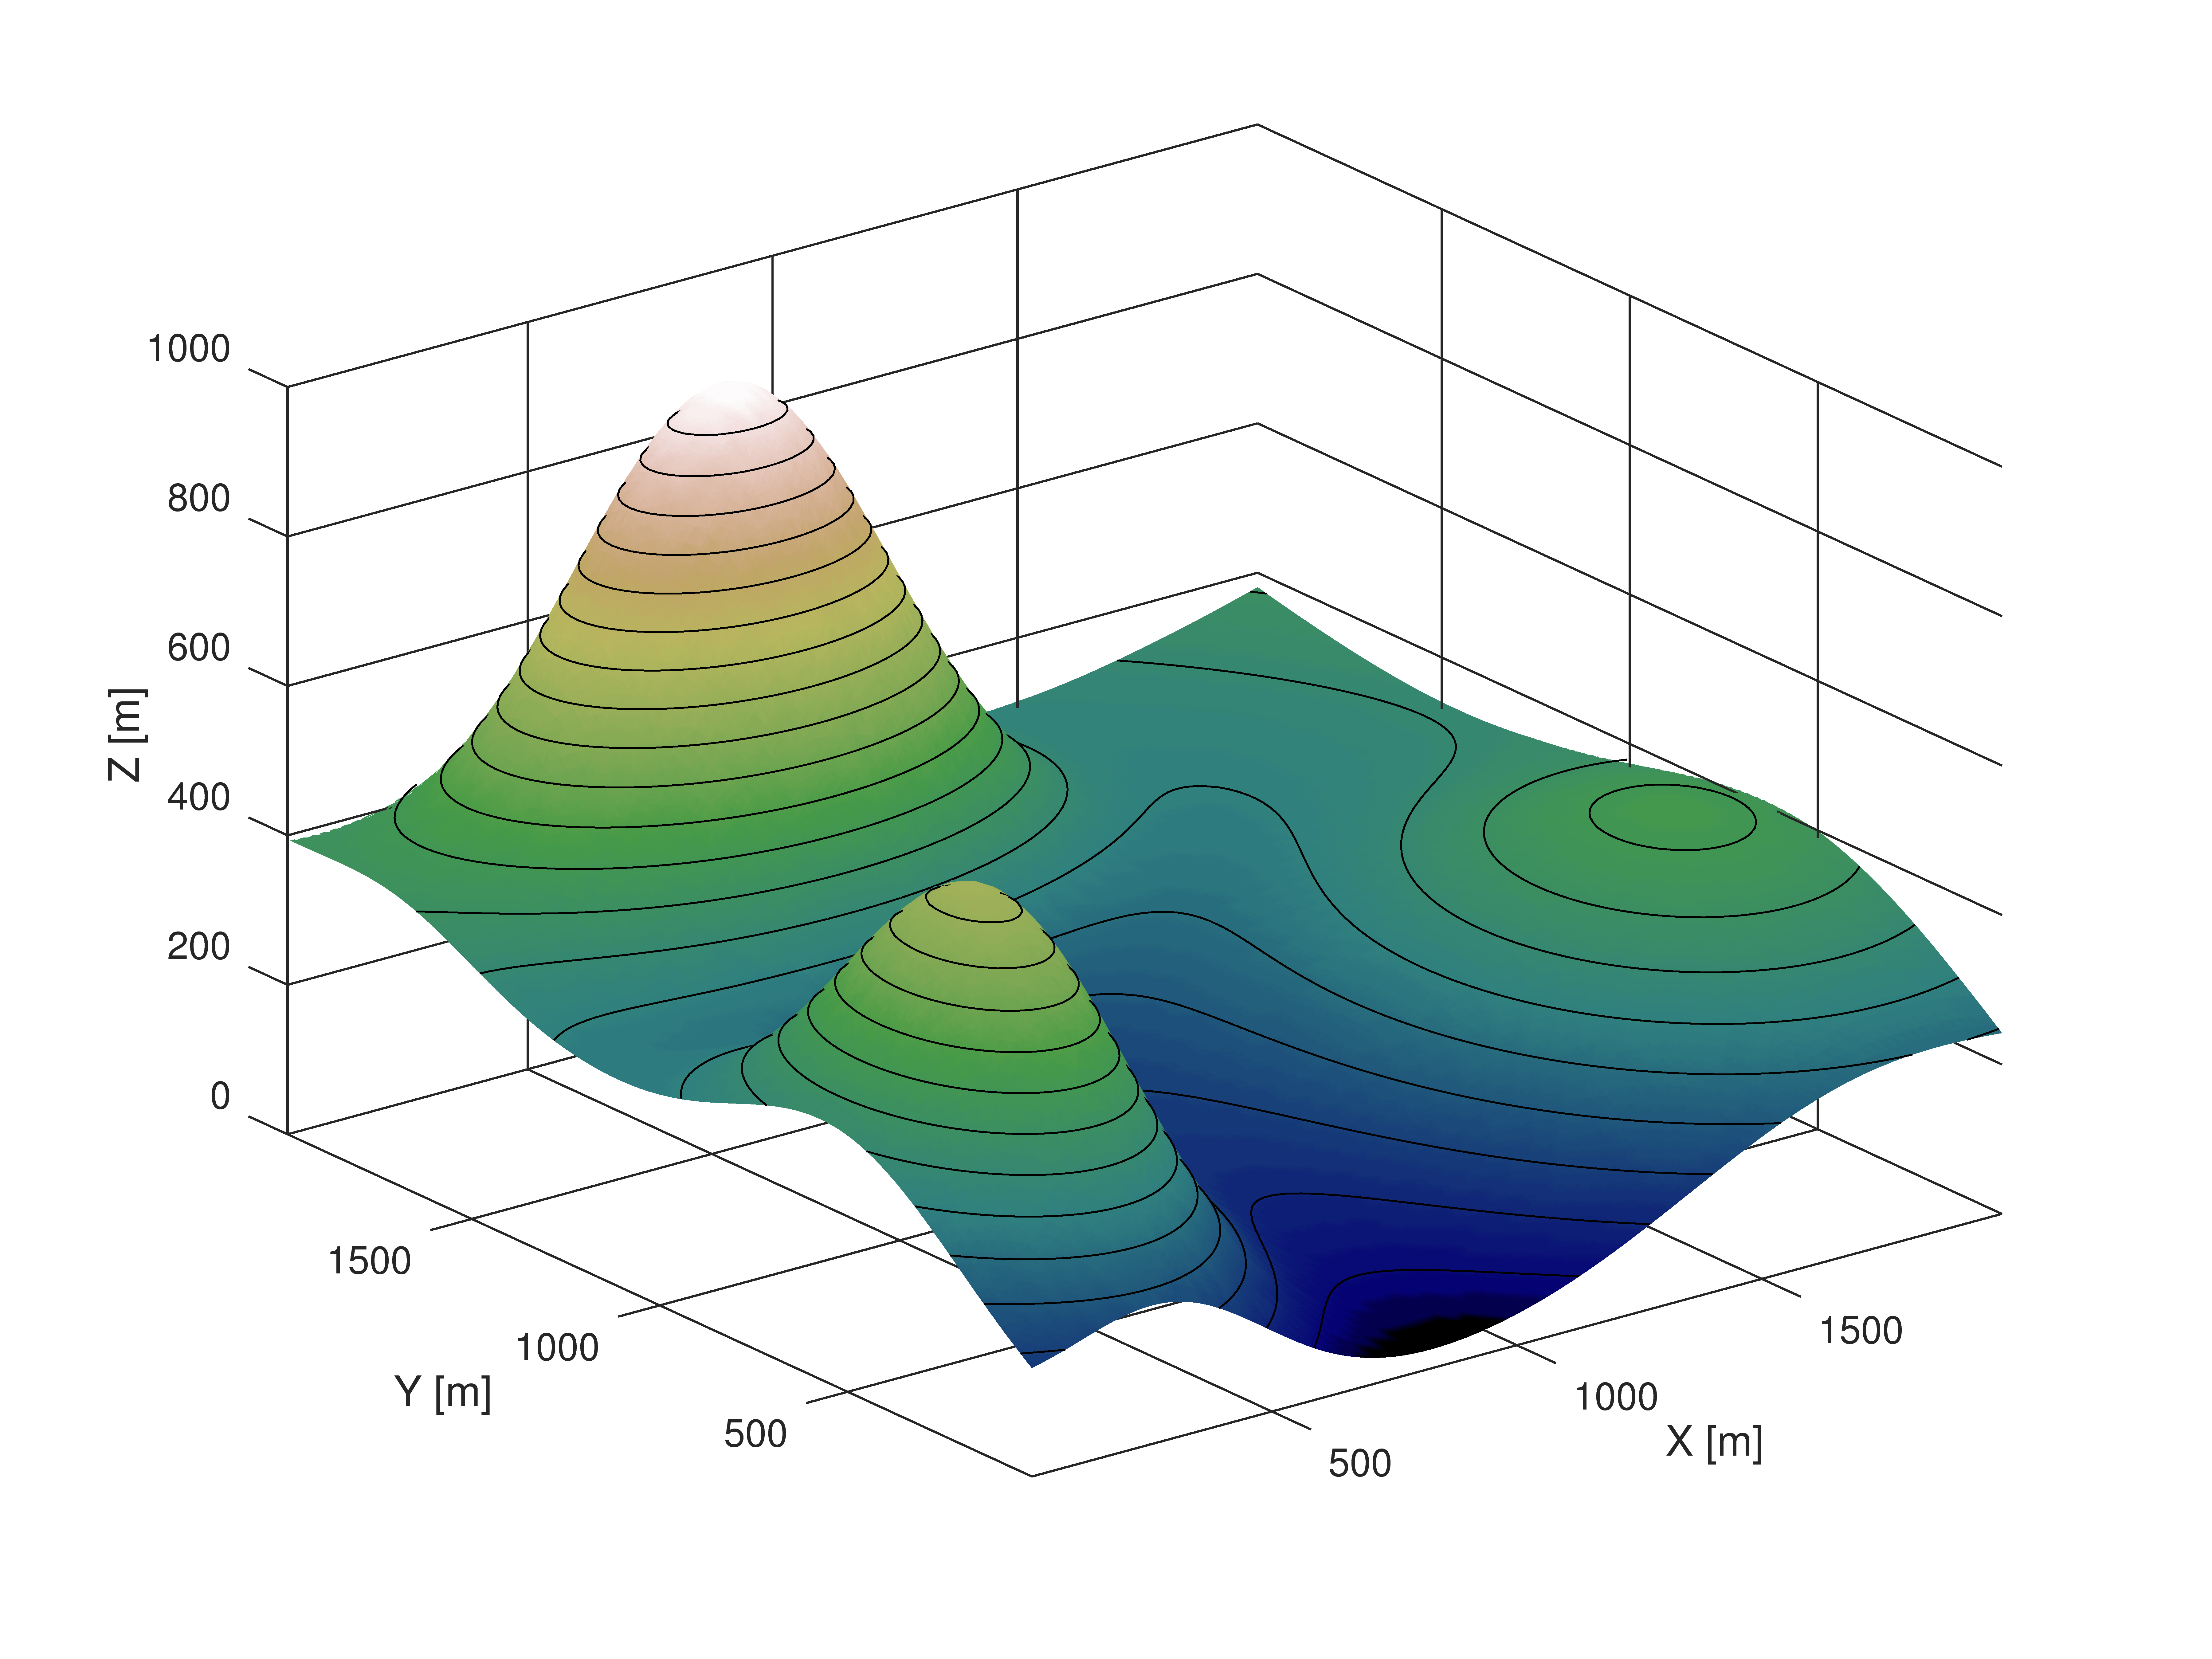
\includegraphics[width=0.65\textwidth]{img/topography.png}
    \end{figure}
    \begin{itemize}
      \item rain duration: $6\,[h]$
      \item rain intensity: $10 - 32\,[mm/h]$
      \item soil initial saturation: $\theta_i\,[-]$
    \end{itemize}
  \end{frame}

%%%%%%%%%%%%%%%%%%%%%%%%%%%%%%%%%%%%%%%%%%%%%%%%%%%%%%%%%%%%%%%%%%%%%%%%%%%%%%%%
% TASK 2 - Results simulations
\section{Task 2}
  \begin{frame}
    \frametitle{Task 2 - Simulations results}
    \begin{figure}[t]
      \centering
      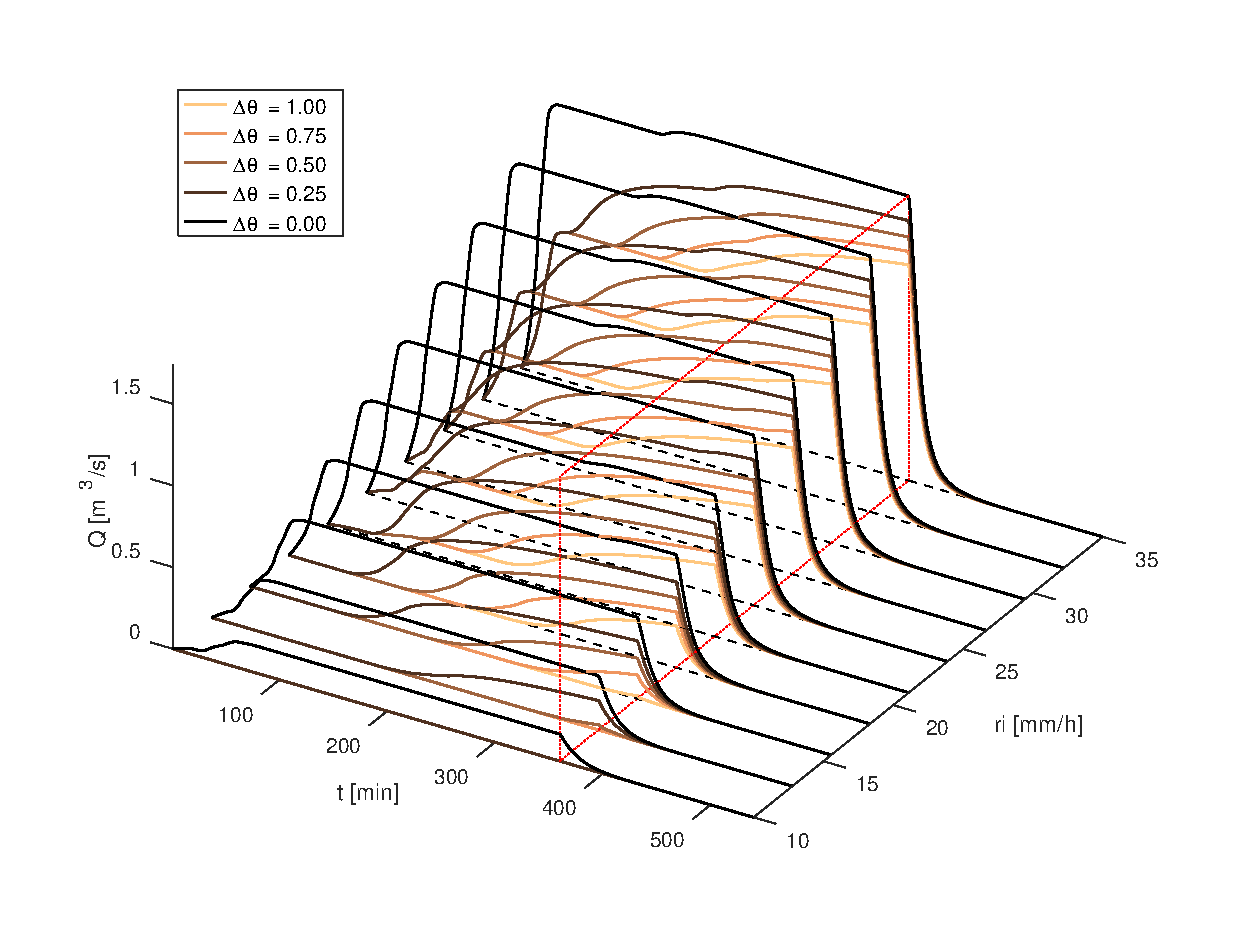
\includegraphics[width=0.75\textwidth]{img/hydrographs3d.eps}
    \end{figure}
    {$Q_{thhold} = 10\,\% \cdot Q_{max}$}
  \end{frame}
  
%%%%%%%%%%%%%%%%%%%%%%%%%%%%%%%%%%%%%%%%%%%%%%%%%%%%%%%%%%%%%%%%%%%%%%%%%%%%%%%%
% TASK 2 - Results emulation - Part 1
\section{Task 2}
  \begin{frame}
    \frametitle{Task 2 - Emulation results}
    \begin{figure}[t]
      \centering
      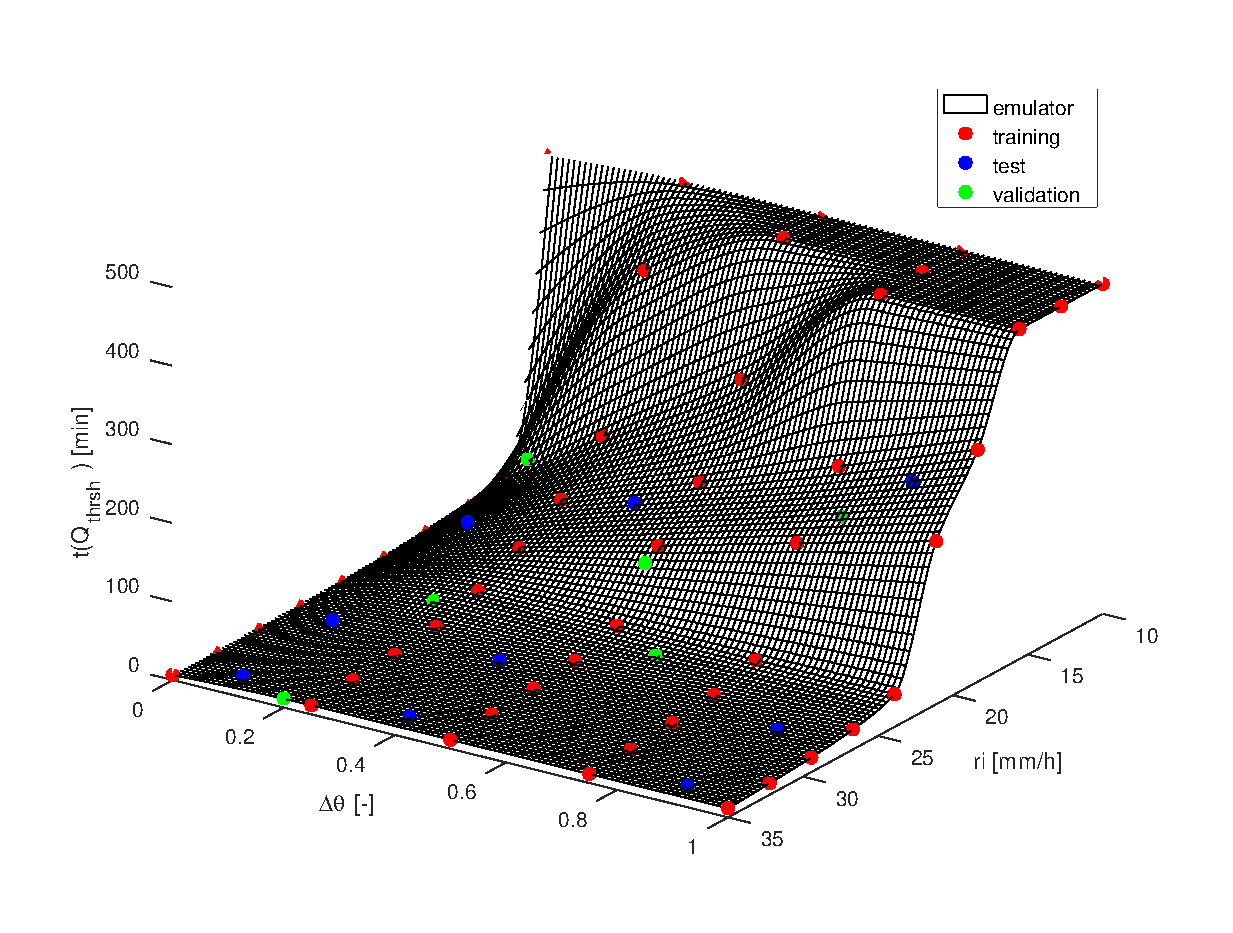
\includegraphics[width=0.8\textwidth]{img/emulator.eps}
    \end{figure}
  \end{frame}
  
%%%%%%%%%%%%%%%%%%%%%%%%%%%%%%%%%%%%%%%%%%%%%%%%%%%%%%%%%%%%%%%%%%%%%%%%%%%%%%%%
% TASK 2 - Results emulation - Part 2
\section{Task 2}
  \begin{frame}
    \frametitle{Task 2 - Emulation results}
    \begin{table}
    \centering
       \begin{tabular}{lcc}
       \toprule
        & \textbf{MAE\,[min, \%]} & \textbf{RMSE\,[min]}\\
       \midrule
       \textbf{1: test} & 5.8, 27.0 & 2.89\\
       \textbf{2: validation} & 11.8, 11.6 & 5.73\\
       \bottomrule
       \end{tabular}
    \end{table}
    \centering
    \large{\textbf{speed-up factor:} \boldmath$1 \cdot 10^5$}
  \end{frame}

%%%%%%%%%%%%%%%%%%%%%%%%%%%%%%%%%%%%%%%%%%%%%%%%%%%%%%%%%%%%%%%%%%%%%%%%%%%%%%%%
% THE END
  {
  \setbeamertemplate{background}{}
  \setbeamercolor{background canvas}{bg=black}
  \setbeamercolor{normal text}{fg=white}
  \usebeamercolor[fg]{normal text}
  \begin{frame}[plain]
    \centering
    \Large{\textbf{THE END}}\\
  \end{frame}
  }

%%%%%%%%%%%%%%%%%%%%%%%%%%%%%%%%%%%%%%%%%%%%%%%%%%%%%%%%%%%%%%%%%%%%%%%%%%%%%%%%
% ADDITIONAL SLIDES
% Links to repositories
  \begin{frame}
    \frametitle{Link to my repositories}
    \small{\url{https://bitbucket.org/binello7/fswof2d}}\\
    \small{\url{https://bitbucket.org/binello7/master_thesis}}\\
    \small{\url{https://bitbucket.org/binello7/master_thesis/wiki/Home}}
  \end{frame}
% ------------------------------------------------------------------------------


\section{Additional slides}
% Weir equation - All experiments
  \begin{frame}
    \frametitle{Weir equation - All experiments}
      \begin{figure}[t]
        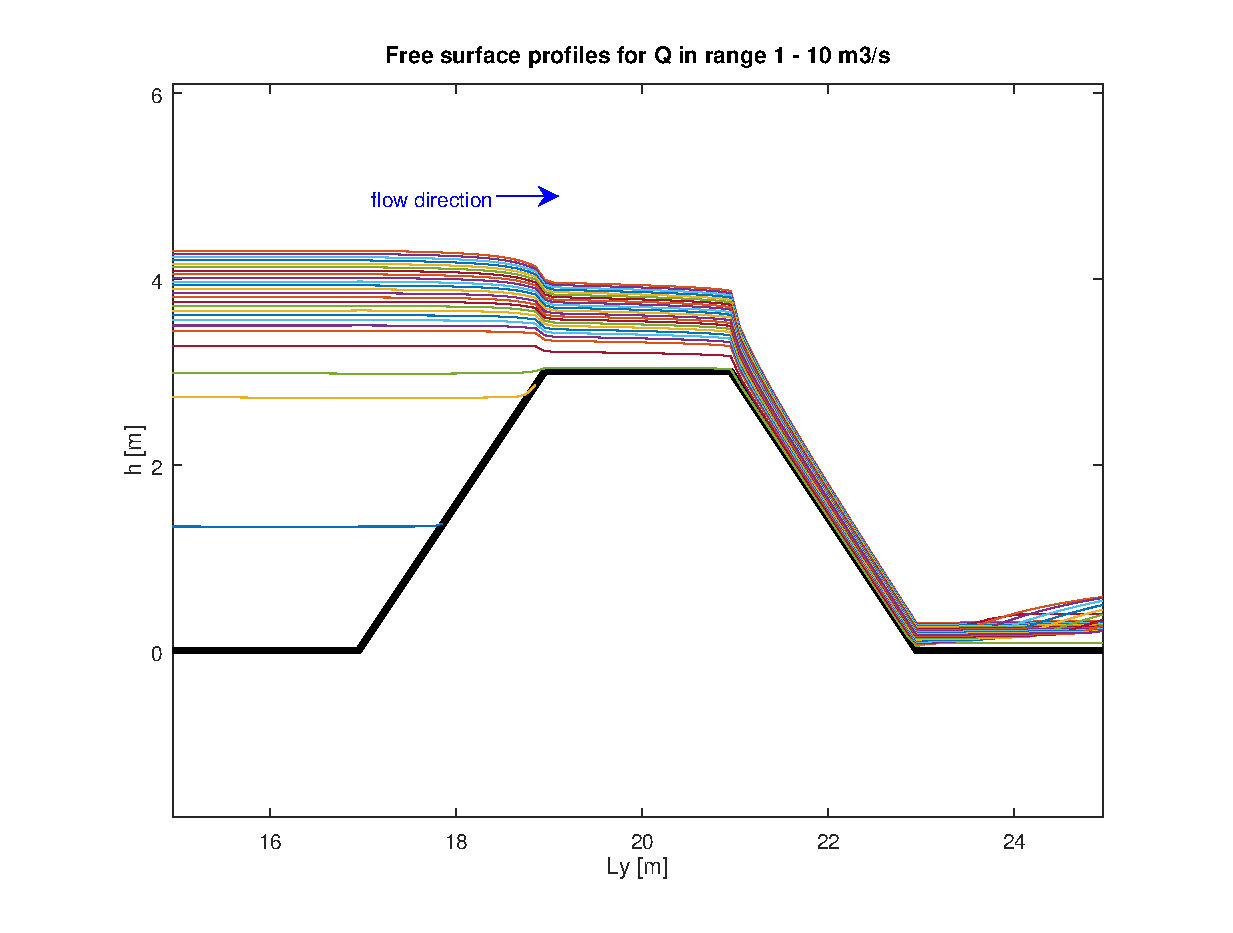
\includegraphics[width=0.5\textwidth]{img/free_surfaces_all.eps}
        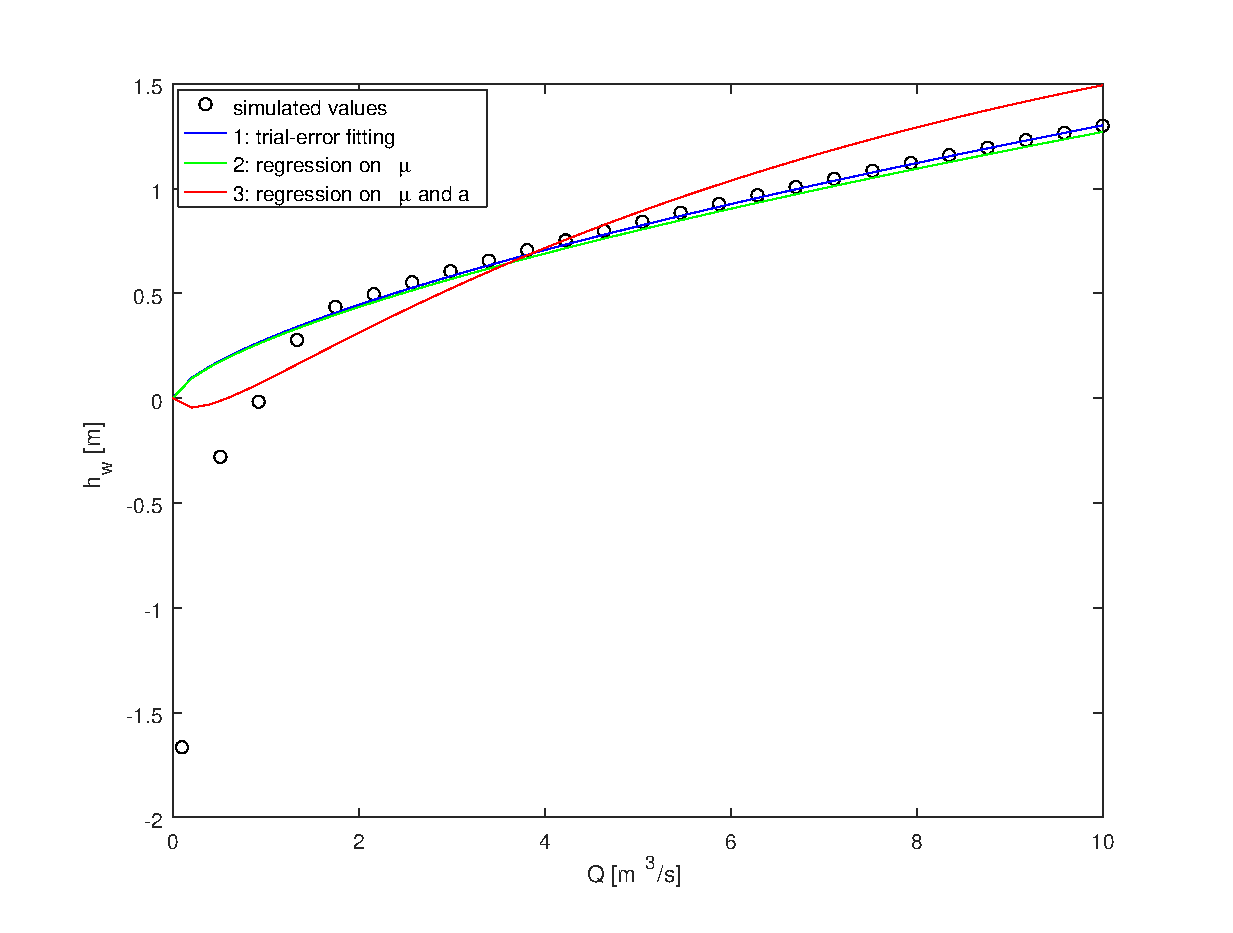
\includegraphics[width=0.5\textwidth]{img/points_interpolations_all.eps}
      \end{figure}
  \end{frame}
% ------------------------------------------------------------------------------

% Validation results emulator
  \begin{frame}
    \frametitle{Emulation resutls: validation}
    \begin{table}
    \centering
    \scalebox{0.9}{
       \begin{tabular}{lcccccc}
         \toprule
         $\Delta\theta\,[-]$ & 0.1 & 0.8 & 0.5 & 0.2 & 0.6 & 0.2\\
         $ri\,[mm/h]$ & 15 & 20 & 22 & 25 & 25 & 35\\
         \midrule
         \textbf{emulator [s]} & 90.25 & 200.00 & 89.70 & 32.67 & 32.90 & 11.22\\
         \textbf{validation [s]} & 91.50 & 192.50 & 101.50 & 32.50 & 32.50 & 11.50\\ 
         \bottomrule
       \end{tabular}}
    \end{table}
  \end{frame}
% ------------------------------------------------------------------------------

% Future possibilities
  \begin{frame}
    \frametitle{Next step}
     \begin{figure}[t]
        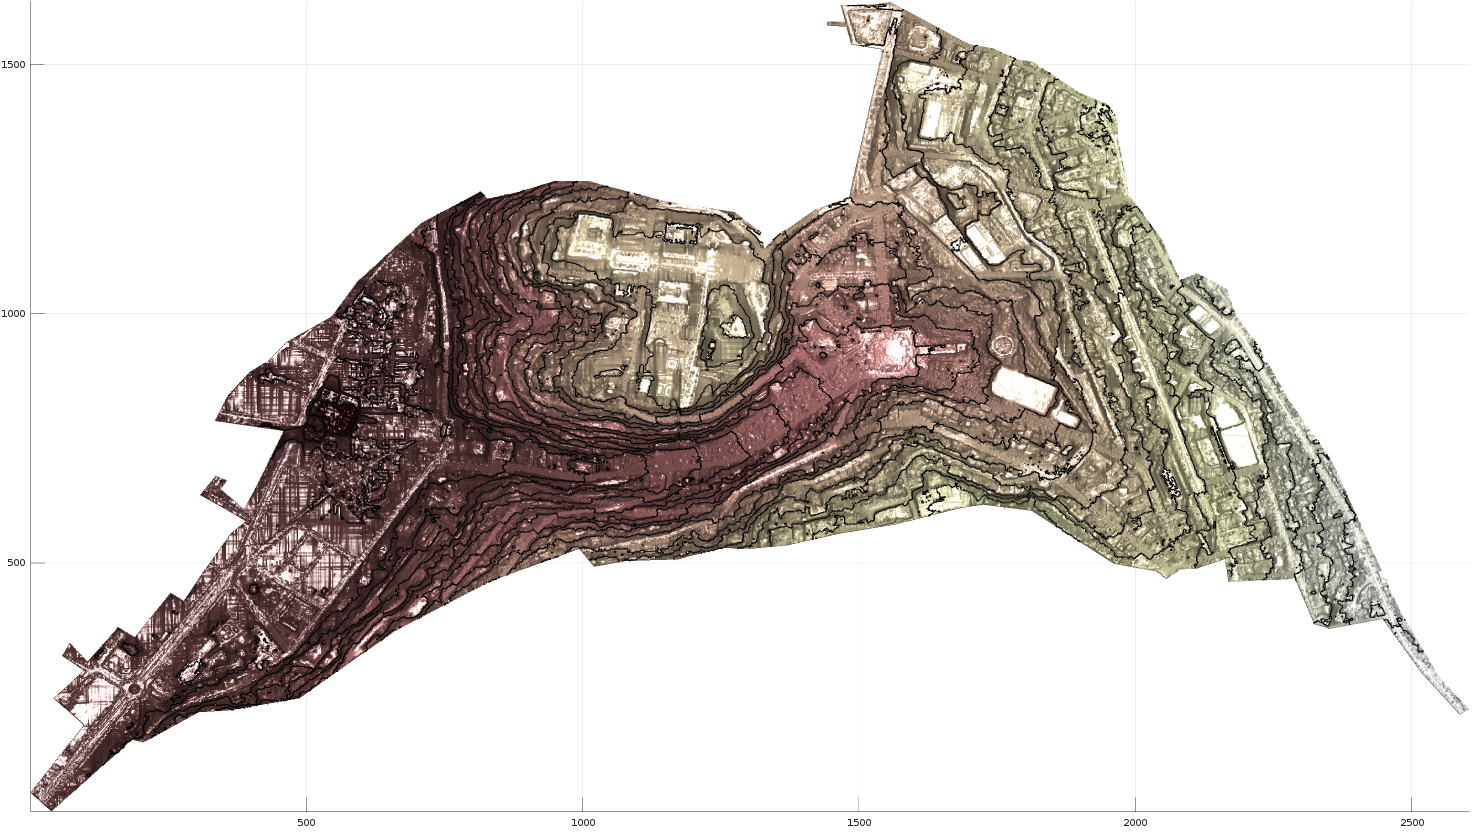
\includegraphics[width=0.5\textwidth]{img/coimbra.png}
        
\includegraphics[width=0.5\textwidth]{img/question.png}
      \end{figure}
  \end{frame}
% ------------------------------------------------------------------------------


\end{document}

